\chapter{Experimental Results}
\label{ch:experiments}

\section{Experimental Design}
\label{sec:expiremental_design}

Following the completion of AFLuent, an evaluation step is needed to understand
how accurate the tool is in localizing faults. This section discusses the design
of this experiment including early steps in choosing and filtering a sample to
test AFLuent on.

\subsection{Approach Overview}
\label{subsec:approach_overview}

In order to evaluate AFLuent, several prerequisites are needed that enable
collecting data for analysis. The primary requirement is a collection of Python
program, which are susceptible of becoming faulty. Additionally, this
collection's complexity must be comparable to code typically written by novice
developers, which AFLuent targets. Another crucial requirement before evaluation
can begin is a test suite for the selected code python code. The test suite must
be executable by Pytest and covers as much as possible of the code under test to
maximize the ability to localize faults. Assuming that these prerequisites are
met and are available, the evaluation of AFLuent can then be generally described
by these four main steps:

\begin{enumerate}
    \item Introduce a bug/fault in the code under test
    \item Run the test suite with AFLuent
    \item Produce a report of suspicious statements as ranked by AFLuent
    \item Asses how far the in the produced ranking report was the location of
    the introduced bug
\end{enumerate}

While these steps are great for planning and describing the intention in evaluating
AFLuent, they fall short of providing a clear and detailed plan. The sections
below will expand on the points discussed here, elaborate on how the
prerequisites are met, and describe the systematic and automated approach in evaluation.

\subsection{Research Questions}
\label{subsec:research_questions_eval}

Before discussing the evaluation process, it's important to clearly state the
questions to answer. Previously, Section\ref{sec:researchq} brought up few
research question concerning the implementation and evaluation of AFL in Python.
Related Work and Methods section addressed \hyperref[para:RQ1.1]{\emph{RQ1.1}} as well as
\hyperref[para:RQ2]{\emph{RQ2}}, however, the answer \hyperref[para:RQ1.2]{\emph{RQ1.2}} remains unclear. While \hyperref[para:RQ1.2]{\emph{RQ1.2}}
generally involved the efficiency and accuracy of AFLuent, there was no mention
of the metrics or the comparisons needed to achieve an answer. In general, there
are sixteen different approaches that will be evaluated and compared. For every AFL
equation used, Tarantula, Ochiai, Ochiai2, and Dstar, there are four tie breaking
approaches. Each equation-tieberaker pair will be evaluated on the same dataset,
where the resulting rankings will be used to produce a score to assess how
close the produced ranking are to localizing the fault correctly. In addition to
this score, the time taken to run each approach will be recorded to compare
their time overhead.

\subsection{Choosing a Sample}
\label{subsec:choosing_sample}

Since AFLuent is targeted towards novice developers with little experience
programming in Python, the evaluation strategy should reflect that by running
AFLuent on novice written code. However, considering that this study does not
involve human subjects, novice developers cannot be asked to write code for the
purposes of this evaluation. To simulate novice written code as best as
possible, the GitHub repository \code{TheAlgorithms/Python}\cite{the_algorithms_python}
is used as the sample. This educational repository is a collection of projects
that implement several fundamental algorithms in Python that range from ciphers,
sorting, graphs, string operations to financial and physics equations.
It resembles novice written
code because, in a sense, beginner developers write these programs while
learning the basics of programming. However, a problem
with using this code is the lack of unit tests that pytest can run, since most
tests are written using Python's doctest. With that in mind, there are Python
tools such as Pynguin\cite{Lukasczyk_Pynguin_Automated_Unit_2022}
that can be used to automatically generate a test suite for these projects.
With the many limitations in Pynguin and the long waiting times to generate
tests, some filtering of the projects is needed.


\subsubsection{Filtering Sample}
\label{subsubsec:filtering_sample}

There are many issues that could arise when automatically generating a test
suite using Pynguin. To mitigate these problems, the following criteria was used
to eliminate entire projects, delete modules, or trim some code.

\begin{itemize}
    \item Projects that import external modules: In order to facilitate and
    expedite generating a test suite using Pynguin, several projects that use
    external packages were removed. These packages include \code{scikit-learn},
    \code{Tensorflow}, \code{Matplotlib}, \code{Sympy}, and \code{PIL}.
    Generating data and creating unit tests for projects that using theses
    packages can be difficult because they are time consuming or simply cannot
    be tested due to their graphical output.
    \item Functions that do not take input or return no results: some implemented
    functions do not accept arguments as input. This makes them difficult to
    test because no data can be passed to them. Additionally, functions that do
    not return a result are also difficult because there is no output to be
    checked. Functions that are part of an object oriented structure that change
    the state of an object without returning a value were kept since their
    results can be tested. However, other functions such as \code{main()} which
    read input from the console and controlled the flow were removed.
    \item Functions with missing type hints in signature: generating data for
    functions with unknown input type would be challenging for Pynguin to
    perform. Therefore, these functions were removed. In some instances where
    the documentation explicitly stated the type of input for the function, type
    hints were manually added to avoid the removal of the function. This was
    especially frequent in sorting function, in which the input was specified as
    integer values.
    \item Code snippets under \code{if \_\_name\_\_ == "\_\_main\_\_"}: In most
    instances the code under this if statement either ran the doctest tests, or
    called a separately implemented main function. Since there is no use for
    these snippets and to clean up the sample, these snippets were removed.
\end{itemize}


\begin{table}[!htb]
    \centering
	\begin{tabular}{|c|c|c|c|}
        \hline
        arithmetic\_analysis & audio\_filters   & backtracking       & bit\_manipulation    \\
        blockchain           & boolean\_algebra & cellular\_automata & ciphers              \\
        compression          & conversions      & data\_structures   & divide\_and\_conquer \\
        dynamic\_programming & electronics      & financial          & genetic\_algorithm   \\
        geodesy              & graphs           & greedy\_methods    & hashes               \\
        knapsack             & linear\_algebra  & maths              & matrix               \\
        physics              & scheduling       & searches           & sorts                \\
        strings              &                  &                    &\\

        \hline
	\end{tabular}
	\caption{Remaining Projects Prior to Test Generation}
	\label{table:remaining_projects}
\end{table}

Following the initial phase of filtering the codebase, general statistics and
observations were recorded for the remaining sample thus far.
Table\ref{table:remaining_projects} shows the name of the remaining project.
Additionally, SLOCcount was used to calculate the number of non-comment line of
code included in the sample. The output from the tool is shown in
Fig\ref{fig:SLOCcount_phase1}. Overall, there was 12199 lines of code remaining
in the sample prior to automatically generating tests using Pynguin.

\begin{figure}[!htb]
	\begin{center}
		\begin{lstlisting}
            SLOC	Directory	SLOC-by-Language (Sorted)
            2396    data_structures python=2396
            1856    ciphers         python=1856
            1583    maths           python=1583
            900     graphs          python=900
            664     sorts           python=664
            559     strings         python=559
            543     conversions     python=543
            412     linear_algebra  python=412
            365     divide_and_conquer python=365
            360     matrix          python=360
            359     dynamic_programming python=359
            308     backtracking    python=308
            248     compression     python=248
            236     searches        python=236
            200     arithmetic_analysis python=200
            173     hashes          python=173
            171     audio_filters   python=171
            161     bit_manipulation python=161
            118     cellular_automata python=118
            109     boolean_algebra python=109
            97      scheduling      python=97
            94      blockchain      python=94
            86      electronics     python=86
            67      genetic_algorithm python=67
            43      financial       python=43
            40      knapsack        python=40
            37      geodesy         python=37
            11      greedy_methods  python=11
            3       physics         python=3

            Totals grouped by language (dominant language first):
            python:       12199 (100.00%)
        \end{lstlisting}
		\caption{\label{fig:SLOCcount_phase1} SLOCcount Output After Initial Filtering}
	\end{center}
\end{figure}


\subsubsection{Generating a Test Suite}
\label{subsubsec:generating_test_suite}

Once initial filtering of the codebase was completed, Pynguin was ran to
generate tests. However, additional issues came up in this process that required
additional filtering to be done. The new content was filtered as follows:
\begin{itemize}
    \item When attempting to generate tests,
    Pynguin failed in 54 modules and threw error messages indicating possible
    bugs in the tool. To limit the time taken to generate tests, 15 minutes were
    given per module, where no tests were generated for 73 modules due to
    getting timed out. Finally, there were 249 modules where tests were
    successfully generated. Modules with failed and timed out runs were removed
    due to the lack of tests that cover them.
    \item Some generated tests were faulty and caused errors when ran, or
    indeterminately failed making them flaky. Those tests were removed in some
    instances or fixed when possible.
    \item Since AFLuent relies on a thorough test suite with high coverage in
    order to find bugs accurately, modules with below 85\% coverage were removed.
\end{itemize}

\begin{figure}[!htb]
	\begin{center}
		\begin{lstlisting}
            SLOC	Directory	SLOC-by-Language (Sorted)
            934     maths           python=934
            826     ciphers         python=826
            576     data_structures python=576
            496     sorts           python=496
            465     conversions     python=465
            454     graphs          python=454
            356     strings         python=356
            217     dynamic_programming python=217
            192     backtracking    python=192
            173     hashes          python=173
            133     bit_manipulation python=133
            101     searches        python=101
            90      linear_algebra  python=90
            69      electronics     python=69
            61      divide_and_conquer python=61
            43      financial       python=43
            42      scheduling      python=42
            37      geodesy         python=37
            27      knapsack        python=27
            16      arithmetic_analysis python=16
            14      cellular_automata python=14
            11      greedy_methods  python=11
            10      compression     python=10
            3       physics         python=3

            Totals grouped by language (dominant language first):
            python:        5346 (100.00%)

        \end{lstlisting}
		\caption{\label{fig:SLOCcount_phase2} SLOCcount Output After Initial Filtering}
	\end{center}
\end{figure}

\begin{figure}[!htb]
	\begin{center}
		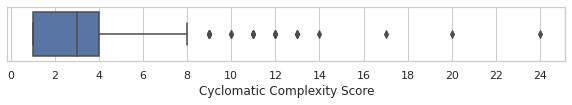
\includegraphics[width=15.5cm]{cyclomatic_complexity.png}
		\caption{\label{fig:cyclomatic_complexity_of_sample} Cyclomatic
		Complextiy of Sample}
	\end{center}
\end{figure}

After the second filtering step SLOCcount statistics were collected again to get
information on the sample, the output from the tool is shown in
Figure\ref{fig:SLOCcount_phase2}. While the codebase was significantly reduced in
size, the resulting test suite contains 1105 test cases with 99\% coverage.
In order to get a better understanding of the remaining sample, additional data
was collected on the cyclomatic complexity the functions in the code. This
information would give some ideas on the structure of the code regarding if
statements, loops and other constructs. The cyclomatic complexity of the
remaining 516 functions was calculated and plotted as shown on Figure
\ref{fig:cyclomatic_complexity_of_sample}. The figure shows a box and whiskers
plot of this data, where the lower quartile and the minimum are equal causing a
lower whisker of zero length. Additionally, the plot shows a median cyclomatic
complexity score of 3 and a maximum of 8. Lastly, few data outliers go beyond
and up to a score of 24. These results mean that the code is very linear, they also suggest that it resembles
what novice developers write as simple only block function and minimal branching.

\section{Evaluation}
\label{sec:evaluation}

\subsection{Data Collection}
\label{subsec:data_collection}

After choosing and filtering the sample, the evaluation of AFLuent would be
conducted by repeating three main steps: (1) Introduce a single bug in the codebase,
(2) Run AFLuent expecting the tests to fail, and (3) collect the reports
produced by AFLuent for analysis later on. With the large sample and the
possibility of inserting bugs in many possible locations, there was a need for
an automated approach to collect this data. Some existing tools such as
\emph{mutmut}\cite{mutmut} already perform similar steps for
mutation testing and it could be easily repurposed to generate the bugs/mutants and run
AFLuent after inserting a mutant into the codebase. Futhermore, \emph{mutmut}
supports a hook function that facilitates collecting results after each run and
before the next mutant is applied. Lastly the test suite run command can be
modified to run AFLuent in evaluation mode and collect fault localization data.
Overall, for each bug/mutant, the following data would be collected to use for
evaluation:
\begin{itemize}
    \item Statement rankings produced by AFLuent for each 16
    approach-tiebreaker combination. Note that a value of 3 was used for * in
    the DStar equation.
    \item Per-test coverage report
    \item Timing report containing the time taken to run the test suite befor
    fault localization and the time to perform fault localization and get
    rankings.
    \item Information about the mutant such as the file and line number it was
    added to as well as the mutated code.
\end{itemize}

AFLuent ranking and timing data was collected on five different machines each with
Ubuntu operating system, \code{Intel Xeon E3-12xx} CPU, and 2GB of memory. Docker containers were created
on each machine, where Python 3.10.2 was installed along with AFLuent and
\code{mutmut}. After running \emph{mutmut} on the filtered algorithms, it was able
to generate 7767 mutants in which 4123 were killed, 3490 survived, and 154 were
timed out by \code{mutmut}. The mutants were classified using the following criteria:

\begin{itemize}
    \item Killed mutants: cases where the mutated code caused a failure in the
    test suite, as expected, prompting AFLuent to localize the fault and
    generate ranking reports.
    Every mutant that generated the ranking reports is
    considered killed.
    \item Survived: cases where the mutation did not cause a failure in the test
    suite. AFLuent was not run in these cases since no test case failed. Runs
    that generated per-test coverage and timing reports but no ranking reports
    are for mutants that survived.
    However, per-test coverage and timing reports were generated.
    \item Timed out: special cases where \emph{mutmut} reported to run a mutant
    but no report was produced by AFLuent. The log produced by \code{mutmut}
    confirms that these mutants were timed out after taking too long to complete
    the test run.
\end{itemize}

When evaluating AFLuent's effectiveness in ranking lines of code, only the
results from killed mutants are relevant since that's when reports were
generated. As for efficiency evaluation, data can be split up to two categories,
time taken by AFLuent to execute tests while calculating per-test coverage, and
time taken to produce rankings to find faults. Both types of mutants, killed and
survived, produced data points on the time taken to run the tests. However, only
killed mutants can produce data points on the time taken to perform
localization. Therefore, a different number of data points will be used for each
category.

\subsection{Results}
\label{subsec:eval_results}

The collected data is visualized in this subsection to compare the different
equations to each other, additionally, tie breaking techniques are compared to
determine the most effective. In order to quantify the effectiveness of each
approach, an \emph{EXAM} %TODO: add citation
score is calculated for each report produced from a killed mutant. This score
represents the percentage of reported statements that a developer must parse
through before reaching the correct line where the bug exists. To produce this
score, the reported results were filtered by project so that the reported
results only include lines from that project. For example, when the \emph{EXAM}
score is calculated for a fault in the \code{bit\_manipulation} project, the
percentage of lines belonging to that project that a developer must read before
finding the fault is the score. The lower the exam score for an approach, to
more effective it is because the developer would have to analyze less lines
before finding the fault.

To visualize the data, box plots are
used to show the distribution of scores for each equation-tiebreaker
combination. This form of visualizing the data allows each point to be
represented in the graph and gives a clear indicator of where outliers are.
Additionally, heat maps are used to compare each pair to the other fifteen after
completing statistical tests.

\subsubsection{Data Vizualization}
\label{subsubsec:data_vizualization}

To compare suspiciousness score equations when the tie breaking approach is the
same, Figures \ref{fig:random_tiebreak_boxplot},
\ref{fig:cyclomatic_tiebreak_boxplot}, \ref{fig:logical_tiebreak_boxplot}, \ref{fig:enhanced_tiebreak_boxplot}
group \emph{EXAM} scores by tie breaking technique for each killed mutant. On
each plot, the y-axis contains the name of the approach and the x-axis the
percentage of score to be analyzed before finding the mutant (also referred to
as the \emph{EXAM} score). Additionally, the value of the median is labeled on
each boxplot. Lastly, outliers are shown using the black circles that go beyond
the limit of the upper whisker on each plot.

\begin{figure}[!htb]
	\begin{center}
		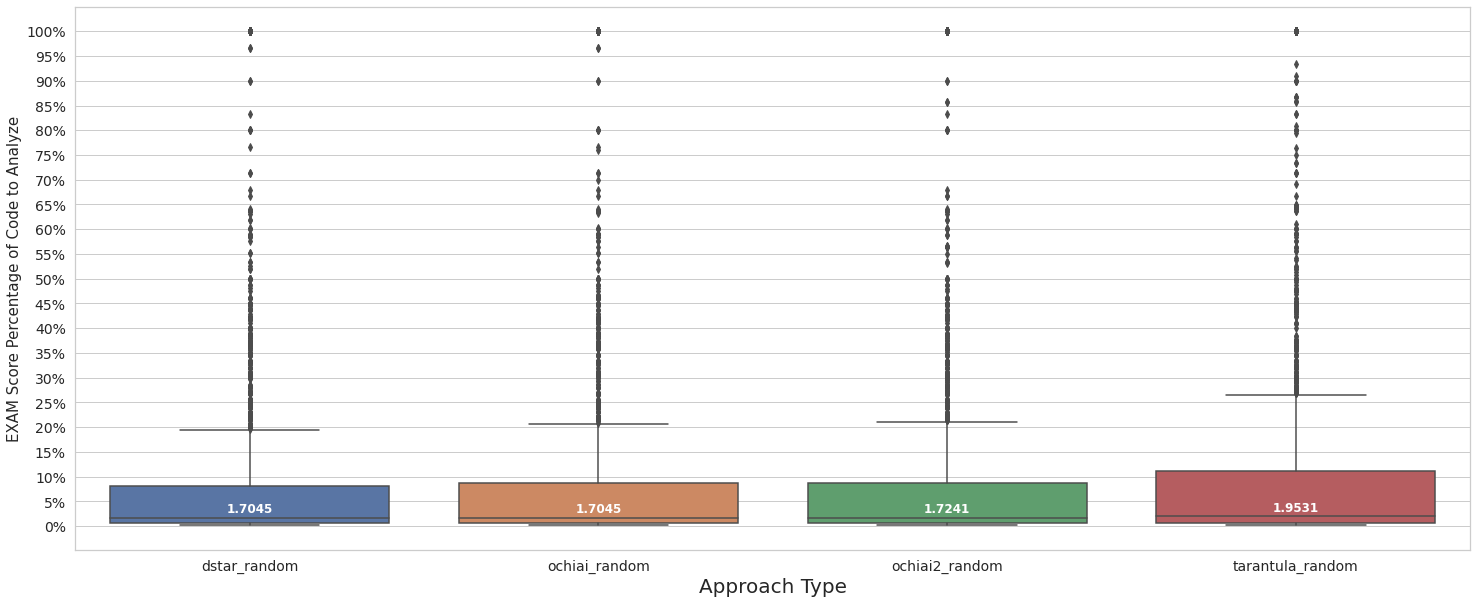
\includegraphics[width=15.5cm]{random_tiebreak_boxplot.png}
		\caption{\label{fig:random_tiebreak_boxplot} \emph{EXAM} Scores Using
		Random Tiebreaking}
	\end{center}
\end{figure}

\begin{figure}[!htb]
	\begin{center}
		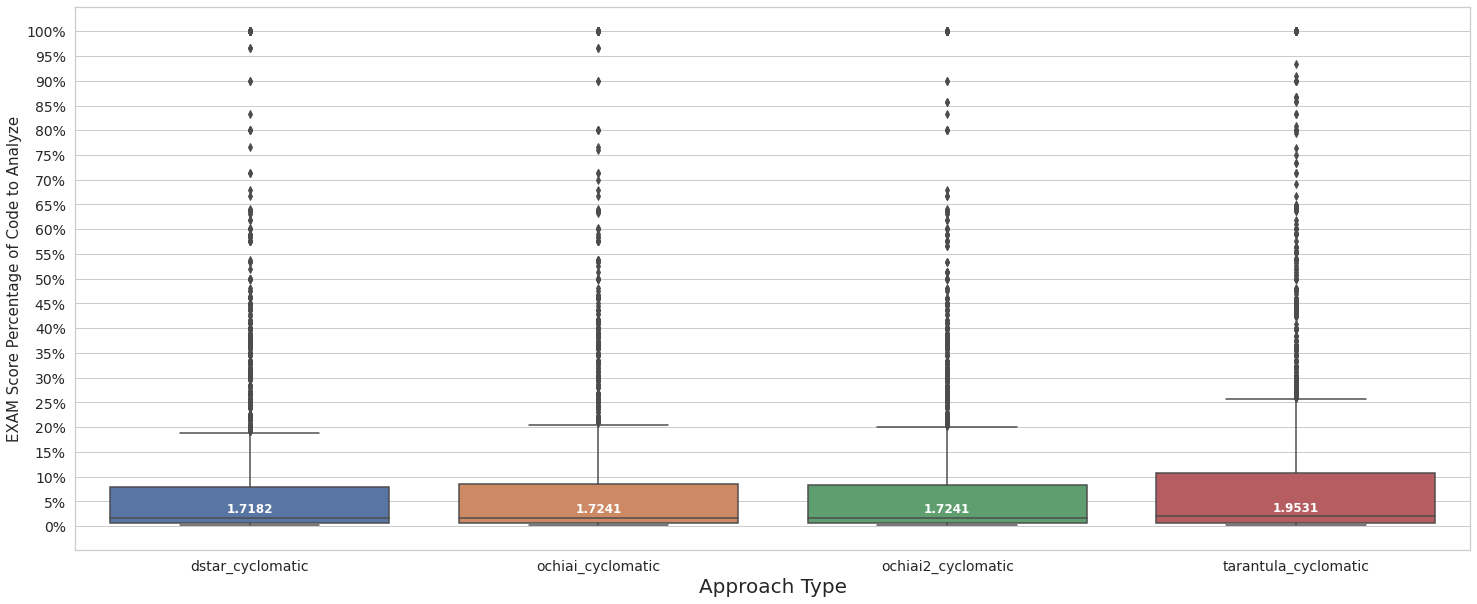
\includegraphics[width=15.5cm]{cyclomatic_tiebreak_boxplot.png}
		\caption{\label{fig:cyclomatic_tiebreak_boxplot} \emph{EXAM} Scores Using
		Cyclomatic Tiebreaking}
	\end{center}
\end{figure}

\begin{figure}[!htb]
	\begin{center}
		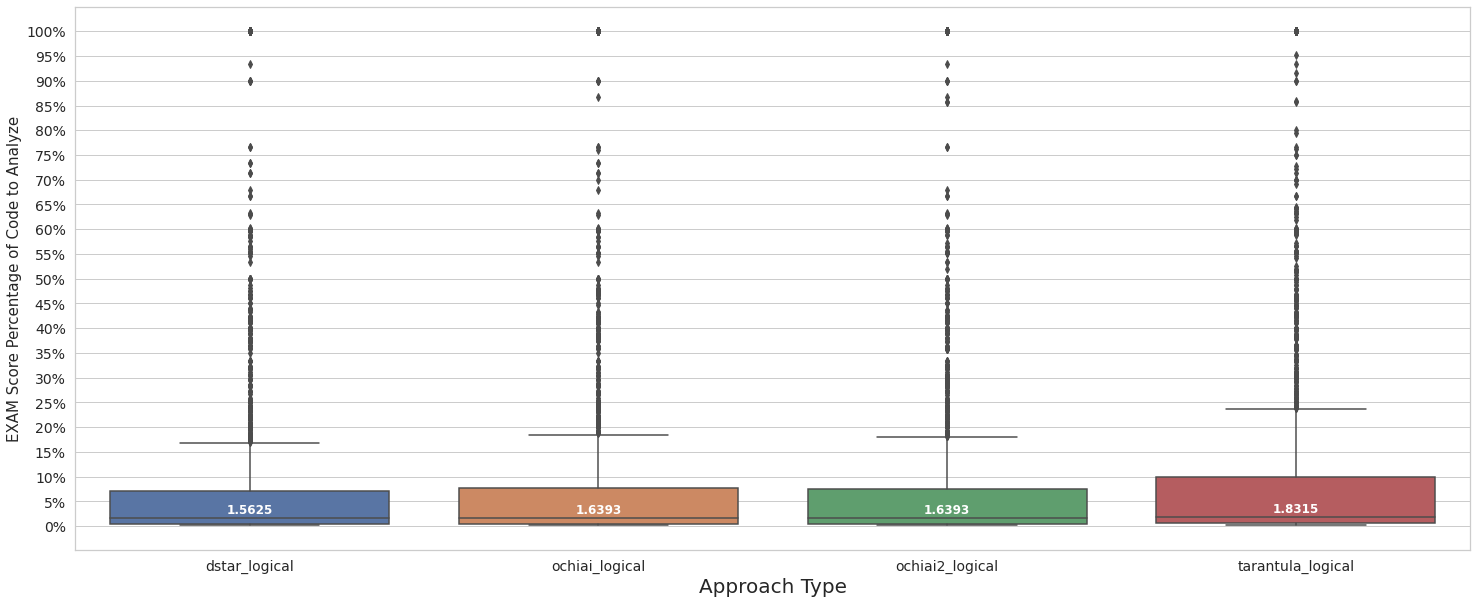
\includegraphics[width=15.5cm]{logical_tiebreak_boxplot.png}
		\caption{\label{fig:logical_tiebreak_boxplot} \emph{EXAM} Scores Using
		Logical Tiebreaking}
	\end{center}
\end{figure}

\begin{figure}[!htb]
	\begin{center}
		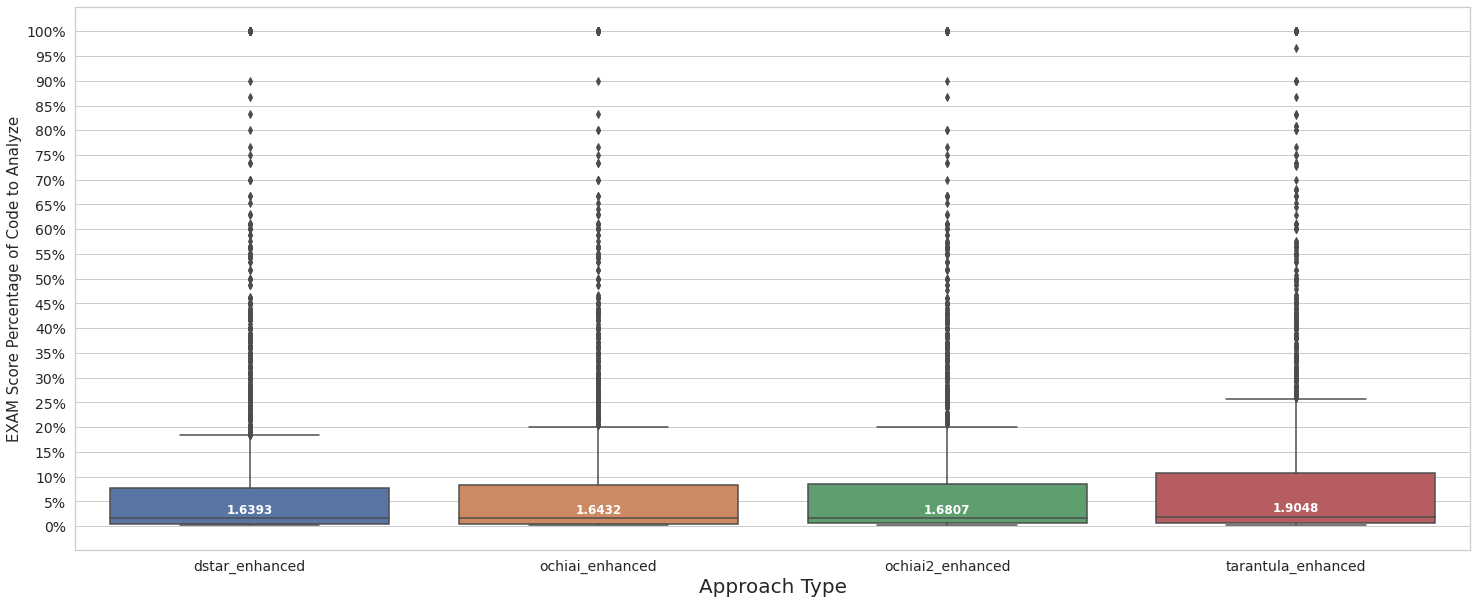
\includegraphics[width=15.5cm]{enhanced_tiebreak_boxplot.png}
		\caption{\label{fig:enhanced_tiebreak_boxplot} \emph{EXAM} Scores Using
		Enhanced Tiebreaking}
	\end{center}
\end{figure}

In Figure \ref{fig:random_tiebreak_boxplot}, which compares the four
equations using random tie breaking, one noticeable difference between the
equations is in the Tarantula approach which has the highest median of 1.9531.
Additionally, it has the highest maximum \emph{EXAM} score around 26\%.
Out of the remaining equations in the plot, DStar and Ochiai have the same
median, however, DStar has a lower maximum making it slightly the better
equation. From visually inspecting the data in Figure
\ref{fig:random_tiebreak_boxplot}, DStar appears to be the most effective, while
Tarantula is the least effective in fault localization. So far, this only
applies when ties are handled randomly.

Moving on to Figure \ref{fig:cyclomatic_tiebreak_boxplot}, improvements in the
median are not noticeable. In fact, the median for DStar and Ochiai is higher
using cyclomatic tie breaking when compared to random tie breaking. The general
trend in the effectiveness of the equation stays the same from the previous
figure, where DStar was the most effective and Tarantula was the least
effective. However, Figure \ref{fig:cyclomatic_tiebreak_boxplot} could suggest
that breaking ties using cyclomatic complexity is no better than randomly doing
so. But, further statistical analysis is needed to come to that conclusion.

When analyzing Figure \ref{fig:logical_tiebreak_boxplot}, there is a noticeable
visual difference to the previous plots. Specifically, the the median
\emph{EXAM} score for all approaches using logical tie breaking is smaller when
compared to random and cyclomatic tie breaking. While this implies an
improvement, it's still unclear if it's statistically significant. In addition
to smaller score medians, approaches using logical tie breaking have smaller
maximums. As for outliers, some differences are present, where there are small
shifts downwards in their values, further implying the improvement that logical
tie breaking provides. As for the rankings between the equations, Tarantula
still appears to be the worst performing while DStar has the lower scores
overall.

Lastly, \emph{EXAM} score while using enhanced tie breaking are shown in Figure
\ref{fig:enhanced_tiebreak_boxplot}. When comparing the results of this figure
to those in Figure \ref{fig:logical_tiebreak_boxplot}, the median values as well
as maximums appear to be higher. This indicates that enhanced tie breaking might
not be as effective as logical tie breaking. However the enhanced approach still
seems as an improvement to the random and cyclomatic ones. The rankings of the
approaches remains the same as the previous three figures, where DStar has the
lowest overall scores and Tarantula has the highest.

Throughout the last four figures, it appears that Ochiai and Ochiai2 have
generally performed the same, with Ochiai2 having slightly higher median in some
cases. This is quite surprising considering that Ochiai2 is considered an
improvement on Ochiai. Overall, both of them have had the same maximum abd
similar distribution in outliers. From visual analysis of the plots, it's
unclear which is more effective.

In addition to the box plots that showcase the medians, and the quartiles, it's
worth looking at the average exam score for each approach. Figure
\ref{fig:averages_barplot} plots the \emph{EXAM} score averages for all
categories. This barplot further demonstrates the low performance of Tarantula,
in which it has the highest averages out of all other equations. Based on the
averages in the plot, the best performing approach is DStar with logical tie
breaking with an average of 18.27\% \emph{EXAM} score. It's followed by Ochiai
logical and Ochiai2 logical with very close averages.

\begin{figure}[!htb]
	\begin{center}
		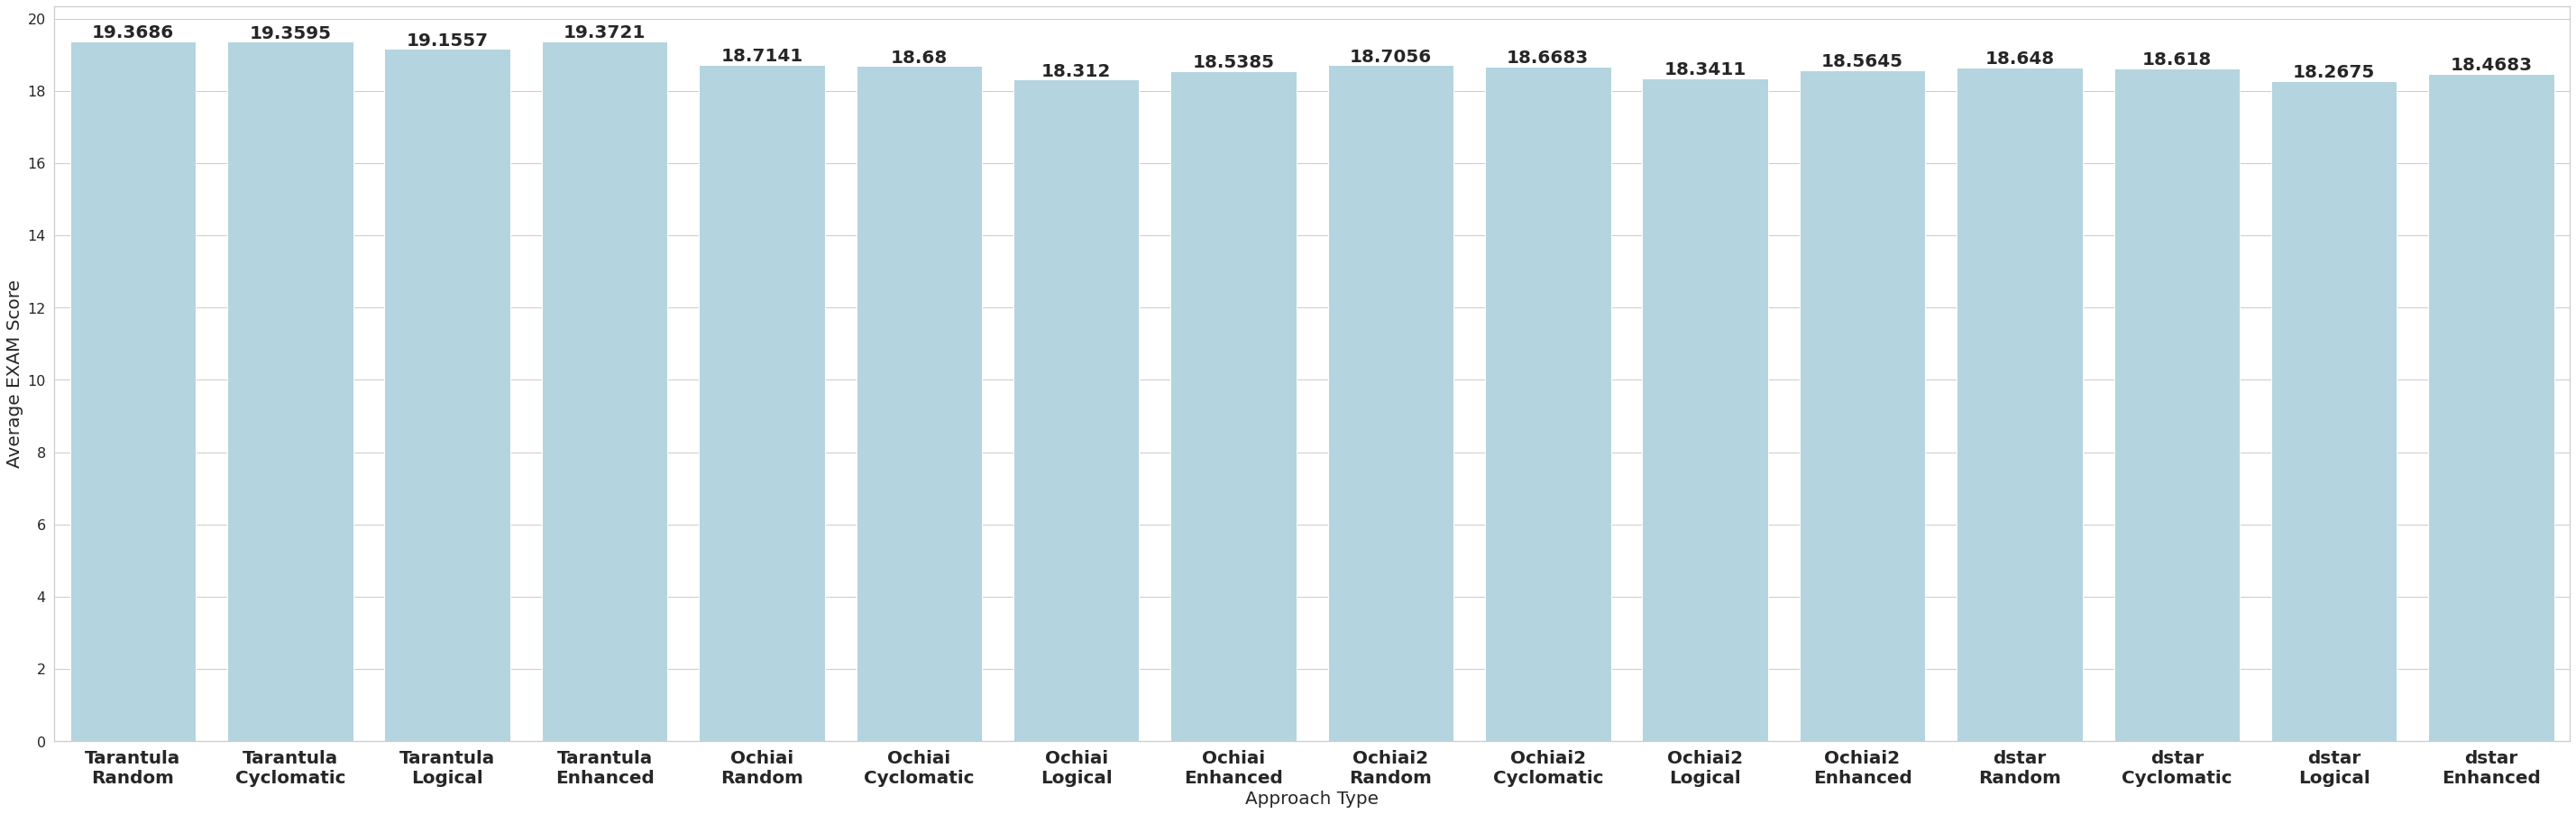
\includegraphics[width=15.5cm]{averages_barplot.png}
        \caption{\label{fig:averages_barplot} Average \emph{EXAM} Scores for all
        Approaches}
	\end{center}
\end{figure}

\subsubsection{Statistical Tests: Mann-Whitney}
\label{subsubsec:statistical_test_mann_whitney}

Simple visual analysis of the data is not enough to reach a justifiable results
regarding the most effective approach. Therefore, this subsection discusses how
two statistical tests were conducted to compare all 16 different approaches to
each other. Starting with the Mann-Whitney U Test, it is used to test whether
the distributions of two independent samples are equal or not. In the two-sided
Mann-Whitney test, the hypotheses are as follows:
\begin{center}
    Null hypotheses: \textbf{H$_{0}$}: \textbf{A$_{x}$} = \textbf{A$_{y}$}

    Alternative hypotheses: \textbf{H$_{1}$}: \textbf{A$_{x}$} $\neq$
    \textbf{A$_{y}$}
    for \emph{p} $\leq$  0.05

    Where \textbf{A$_{x}$} is the approach on the x-axis and \textbf{A$_{y}$} is
    the approach on the y-axis
\end{center}

The generated p-values from the test represent the probability that
\textbf{H$_{0}$} is true. Therefore, when p-values are less than or equal to the statistically
significant level of 0.05, the test indicates that the two approaches are
statistically different. However, it does not conclude which approach had the
higher or lower exam scores. Figure \ref{fig:two_sided_mw_test} plots a heat map
of the resulting p-values from the two sided Mann-Whitney test. It compares each
approach to the fifteen remaining ones.

\begin{figure}[!htb]
	\begin{center}
		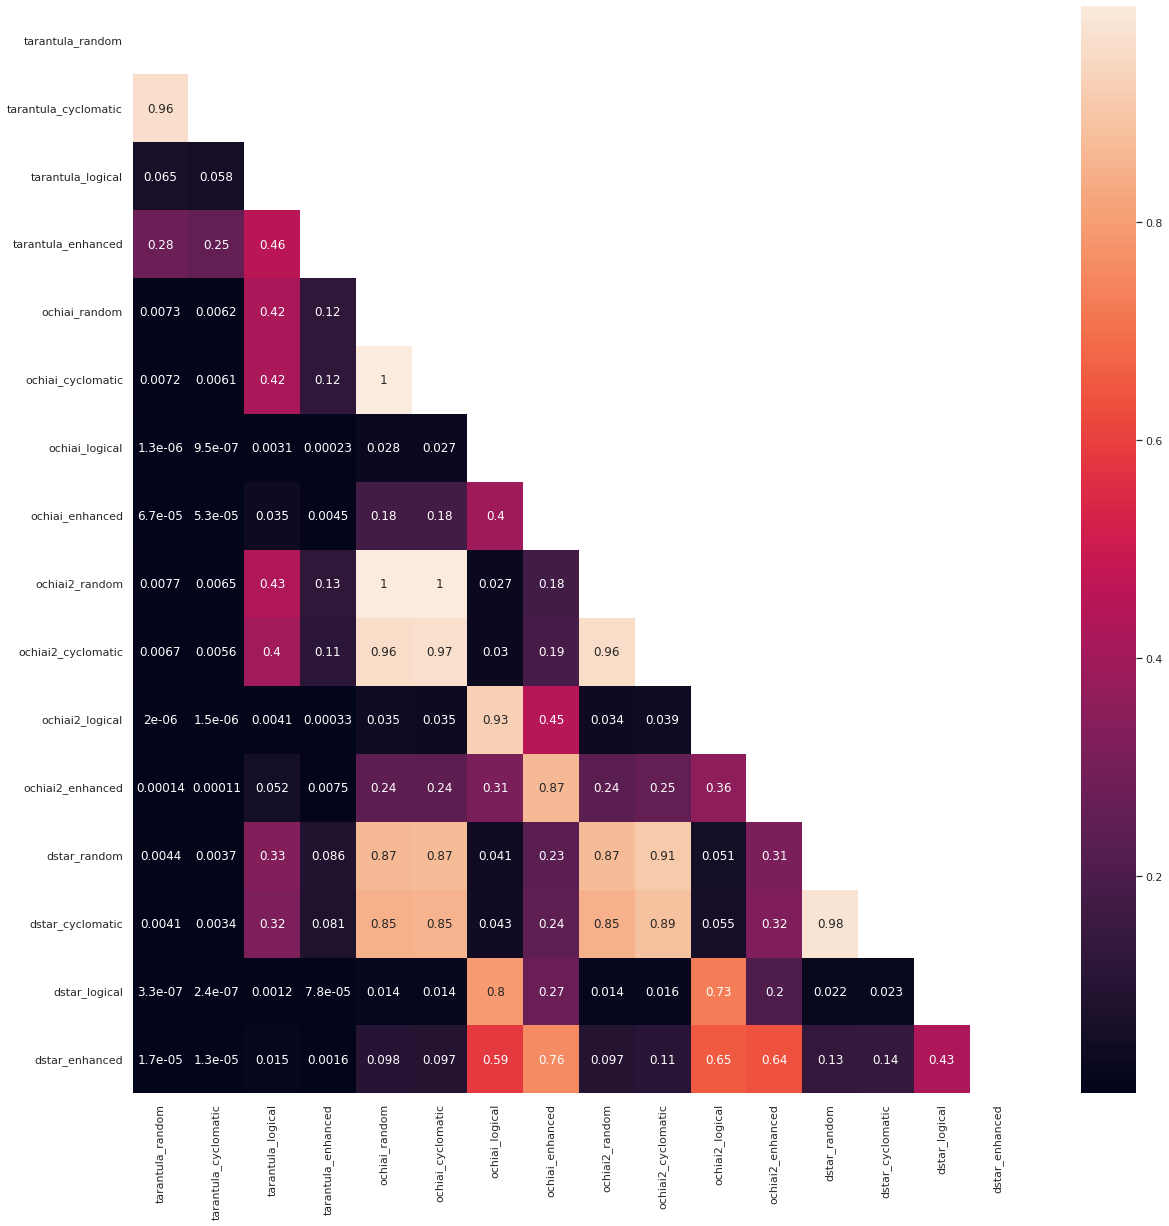
\includegraphics[width=15.5cm]{two_sided_mw_test.png}
        \caption{\label{fig:two_sided_mw_test} P-values of Two Sided Mann-Whitney Test}
	\end{center}
\end{figure}

Many conclusions can be reached from the p-values displayed in the heat map,
some of which further affirm the observations made earlier from the plots, and
others show a completely different result. Starting with the Tarantula
approaches, the p-values for Tarantula clearly
show that these sets are different from all non-Tarantula approaches to a very
statistically significant level.
Therefore, the null hypothesis is rejected
here. There are only few exceptions, where Tarantula Enhanced and Tarantula
Logical are not different from the random and cyclomatic variants of Ochiai,
Ochiai2, and DStar, so the null hypotheses is accepted for these exceptions.
These cases represent an interesting case where using the logical and enhanced
tiebreakers was a significant enough improvement to bring Tarantula in line with
the random and cyclomatic variants of other equations.
When comparing Tarantula variants amongst each other, they aren't statistically
different, therefore, the null hypothesis is
accepted in this case.

For the Ochiai, Ochiai2, and Dstar equations, the heat map shows an interesting
relationship between them. The Random and Cyclomatic variants were very similar,
both across and among each other. For all 15 of these pairs shown in the light
squares in the center of the plot,
\emph{p} was above 0.85 suggesting that the null hypothesis should be accepted.
This result suggests that the different tie breaking techniques were not
effective in giving an equation the edge over another.
As for the remaining variants of Ochiai, Ochiai2, and DStar, namely logical and
enhanced, they are not different from each other on a statistically significant
level. Therefore, the null hypothesis is accepted for these combinations.

While the results of this test are helpful to show if statistically significant
differences exists between the different approaches, it does not clarity which
one is better than the other. To have a better understanding of that
relationship, a one sided \code{less} Mann-Whitney test is performed with the
hypotheses are as follows:

\begin{center}
    Null hypotheses: \textbf{H$_{0}$}: \textbf{A$_{x}$} = \textbf{A$_{y}$}

    Alternative hypotheses: \textbf{H$_{1}$}: \textbf{A$_{x}$} $<$
    \textbf{A$_{y}$}
    for \emph{p} $\leq$  0.05

    Where \textbf{A$_{x}$} is the approach on the x-axis and \textbf{A$_{y}$} is
    the approach on the y-axis
\end{center}

In contrast to the two-sided test, this one gives a more clear idea on which
approaches has a lower \emph{EXAM} scores when compared to others. A \emph{p}
value less than or equal to 0.05 suggests that the approach on the x-axis is
significantly more effective than it's counterpart on the y-axis. On the other
hand, a \emph{p} value greater than 0.95 indicates the opposite, where the
approach on the y-axis is significantly more effective than the one on the x-axis. Figure
\ref{fig:one_sided_mw_test} plots a heat map of the resulting \emph{p} values
from this test.

\begin{figure}[!htb]
	\begin{center}
		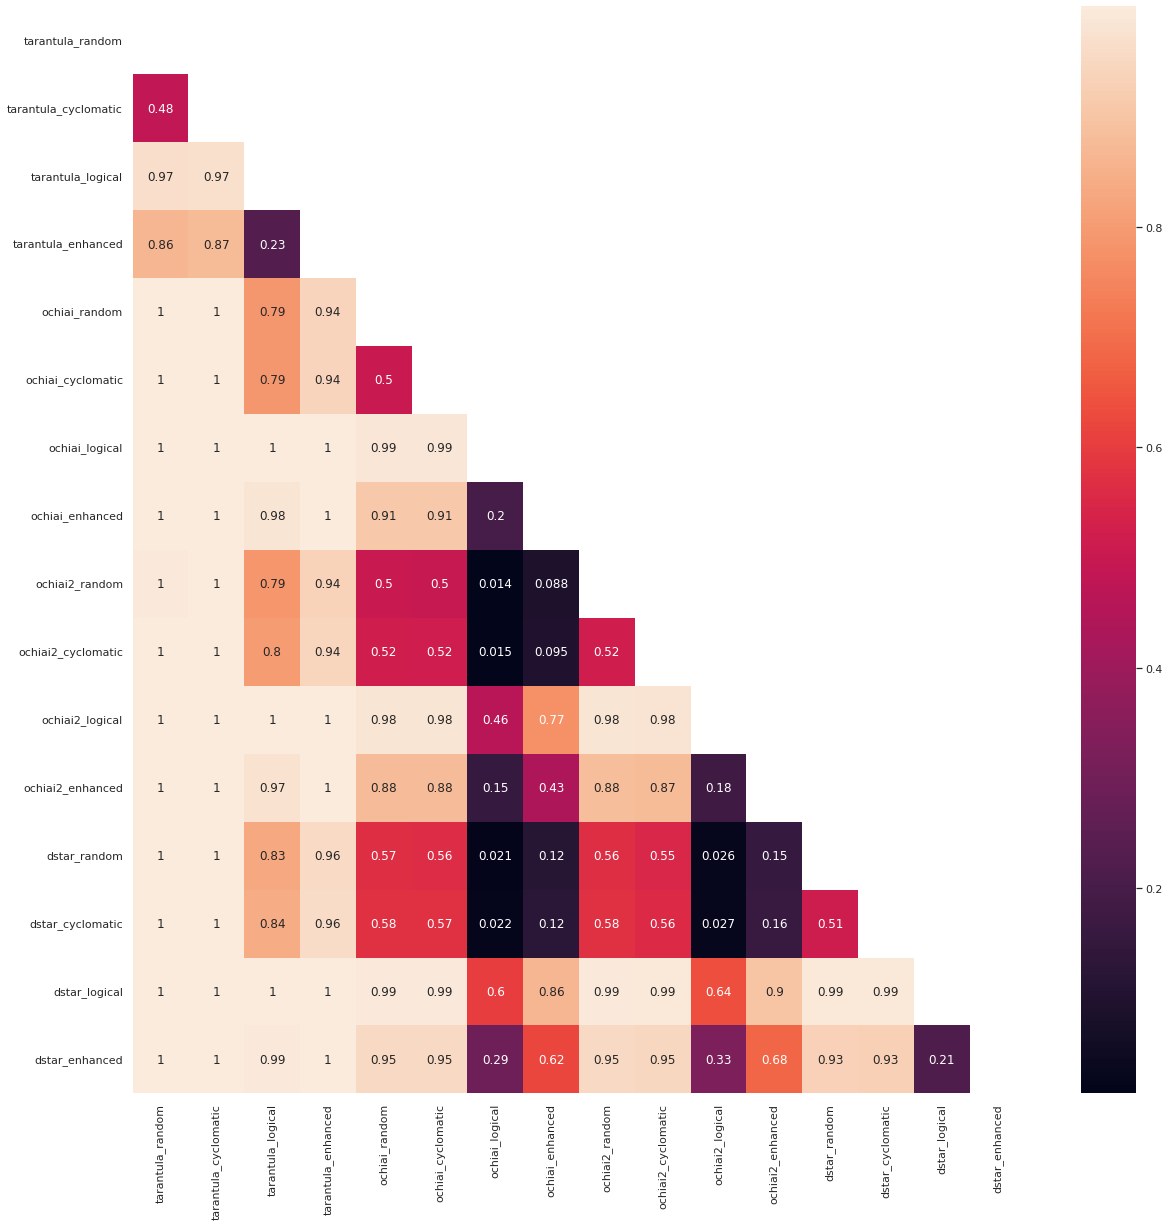
\includegraphics[width=15.5cm]{less_sided_mw_test.png}
        \caption{\label{fig:one_sided_mw_test} P-values of One Sided Mann-Whitney Test}
	\end{center}
\end{figure}

Starting with the Tarantula variants, none of them resulted in a statistically
significant \emph{p} value to suggest that they are more effective than the
other non-Tarantula approaches, thus, the null hypothesis is accepted. However,
among Tarantula variants, the logical tie breakers has the lowest \emph{p}
value, suggesting that it was the most effective but not to a significant level.
To further illustrate how Tarantula falls behind the other equations, every
non-Tarantula approach significantly outperformed the random and cyclomatic
variants of Tarantula. The logical and enhanced variants were also outperformed
by others, however, it was less frequently.

As for other equations, the Random and Cyclomatic variants of Ochiai, Ochiai2,
and DStar all had similar results between each other, where non of them
outperformed another on a significant level. Therefore, for these approaches,
the null hypotheses is accepted. This result matches the outcome of the
two-sided test where these approaches were very similar.

Some notable large differences in performance can be seen in the logical variant
of Ochiai, Ochiai2, and DStar. Theses three significantly outperformed every
random and cyclomatic variant of all other equations. On the other hand, the
enhanced variant of these slightly outperformed the cyclomatic and random ones,
but not on a statistically significant degree. This result suggests that the
logical tie breaker is the most effective in assisting equations to produce the
lowest \emph{EXAM} scores. Furthermore, it demonstrates that while Ochiai and
Ochiai2 do not outperform each other, both show a significant improvement to
almost every other combination.

One of the surprising outcomes of this data is the performance of enhanced tie
breaking. Despite the fact that it adds on the mutant density metric provided by
logical, and considers wider possibility while generating it's score, it did not
outperform the logical tie breaker. In fact, the \emph{p} value was leaning more
to the other outcome, but not in any significant way.

\subsubsection{Statistical Tests: Cohen's D Effect Size}
\label{subsubsec:statistical_test_cohen}

\subsubsection{Time Efficiency}
\label{subsubsec:time_Efficiency}

In order to provide a time comparison that accounts for the different cases of
AFLuent runs, three different categories of time data are included: (I) Time to
execute tests without AFLuent, (II) Time to execute tests with AFLuent enabled,
(III) Time to locate faults and perform tie breaking using all
equation-tiebreaker combinations. Generally all these times were calculated when
all 1105 test cases in the project's suite were ran.

\begin{figure}[!htb]
	\begin{center}
		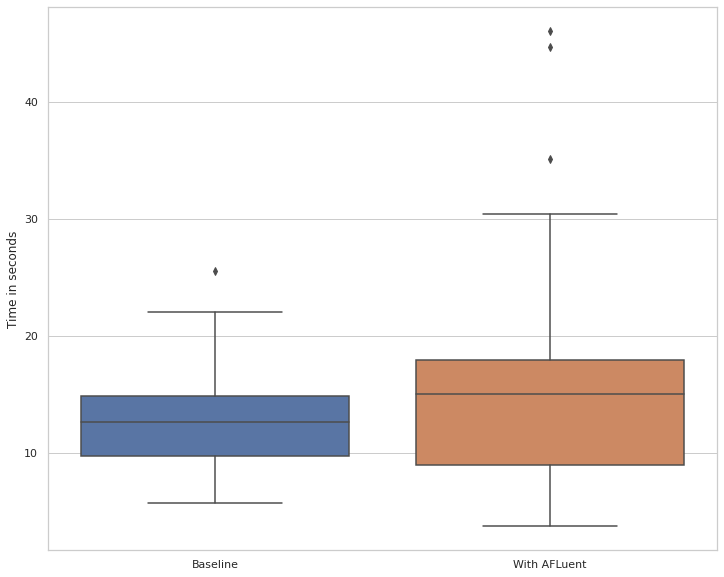
\includegraphics[width=7cm]{test_timings.png}
		\caption{\label{fig:test_timings} Test Execution Time}
	\end{center}
\end{figure}

Figure \ref{fig:test_timings} compares the time taken to execute all test
functions with and without using AFLuent. The baseline includes
4000 data points where the tests were ran without AFLuent. On the other hand
7613 data points are plotted for when AFLuent generated a timing report. The
figure shows a clear difference between the two box plots, where the median run with
AFLuent took longer time to complete than the median run for the baseline.
Additionally, the long upper whisker indicates that
including AFLuent increases the chances that the tests could take substantially
longer to run. This increase is somewhat expected since AFLuent introduces
wrapper functions around each test execution to calculate per-test coverage. And
while this increase is quite small, considering the large size of the test suite,
minimizing the additional time cannot be done through AFLuent since the tool
relies on Coverage.py to calculate per-test coverage. After performing a two-sided
Mann-Whitney Test on both sets, the resulting p-value of
\code{8.035528e-157} confirms that there is statistically significant difference
between the two sets, where the null hypothesis is rejected.

\begin{figure}[!htb]
	\begin{center}
		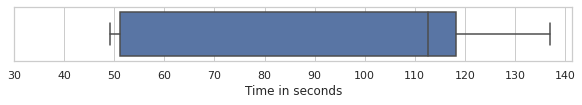
\includegraphics[width=15.5cm]{localization_timings.png}
		\caption{\label{fig:localization_timings} Fault Localization Time}
	\end{center}
\end{figure}

Another useful time metric for developers hoping to use AFLuent is the time the
took takes to locate faults. And while
comprehensive time data for each equation and tie breaking approach was not
collected, some conclusions can be drawn from the most time consuming case.
Figure \ref{fig:localization_timings} shows the time taken to generate a
statement ranking following a test failure. This includes the time to calculate
suspiciousness scores using all equations and to retrieve and evaluate tie
breaking values using all approaches. In general, this is the worst possible
scenario for AFLuent localization time. While the median time is quite large,
around 115 second, so is the test suite. For every run, AFLuent generates and parses
abstract syntax trees using libcst and calculates cyclomatic complexity fo all
files covered in the suite. In the case of this evaluation, this includes all
files in the codebase. Further discussion on how this time can be minimize is
found in Section \ref{sec:future_work}: Future Work.

\section{Threats to Validity}

There are some aspects of this study where the method of collecting data and
performing evaluation could be criticized. In this relatively small scale
evaluation of SBFL equations, the sample chosen to test AFLuent might not
adequately represent code written by novice developers. And while this brings up
the question of how would AFLuent perform on a different type of code base, it
does not completely invalidate the results reached here. The repeated shrinking of the
sample from the original \code{TheAlgorithms/Python} to a very filtered version
can raise several red flags and questions regarding why specific code was
removed. Given the constraints of this study, however, and the intention to
use Pynguin to generate unit automatically, some code had to be removed in order
for Pynguin to run in a timely fashion and produce appropriate tests. It could
be argued that the tests generated by Pynguin were not very thorough, especially
that almost 50\% of the mutants survived while running \code{mutmut}. This
argument brings up a valid criticism and suggests that a well rounded evaluation
of AFLuent requires that the sample be more representative by ensuring that it
was developed by novice developers. Additionally, it indicates that an automatically generated
test suite does not adequately mimics one written by novice developers.
